\begin{frame}{Motivation}
    \begin{itemize}
        \item Les réseaux de neurones récurrents classiques conservent l'information sur une courte durée (une dizaine d'itérations maximum)
        \item \textbf{1991 :} Démonstration de ce problème par la thèse de Sepp Hochreiter (encadré par Jürgen Schmidhuber) \cite{Hochreiter91}
        \item Recherche de solutions à ce problème par Schmidhuber \& Hochreiter
    \end{itemize}
\end{frame}

\begin{frame}{Apparition des LSTM}
    \begin{itemize}
        \item \textbf{1997 :} \citeauthor{Hochreiter97} publient un article nommé \textit{\citetitle{Hochreiter97}} \cite{Hochreiter97} (fig. \ref{lstm1})
        \item \textbf{2000 :} Ajout de la \og forget gate\fg{} au modèle par \citeauthor{Gers00} \cite{Gers00} (fig. \ref{lstm2})
    \end{itemize}

    \begin{columns}
        \begin{column}{0.48\textwidth}
            \begin{figure}
                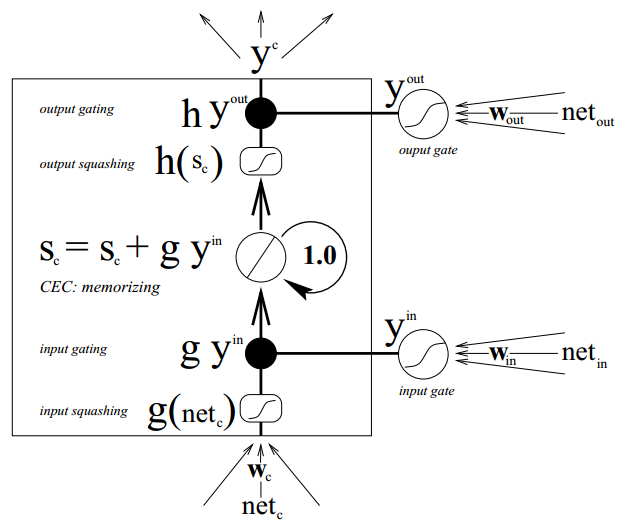
\includegraphics[width=.7\textwidth]{images/lstm1}
                \caption{LSTM orignal}
                \label{lstm1}
            \end{figure}
        \end{column}
        \begin{column}{0.48\textwidth}
            \begin{figure}
                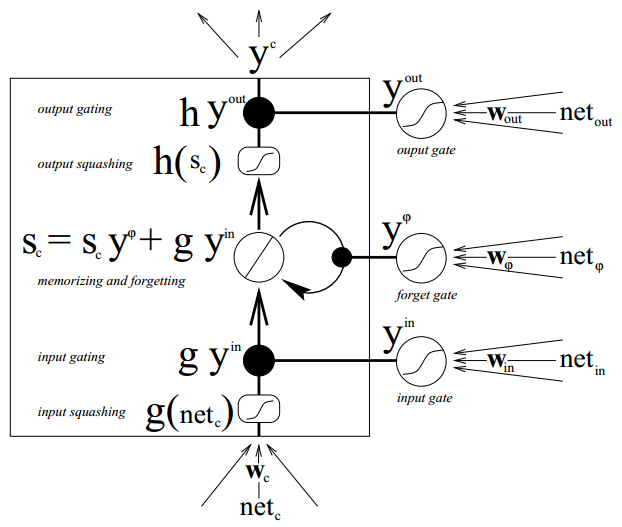
\includegraphics[width=.7\textwidth]{images/lstm2}
                \caption{Ajout de la \og forget gate\fg{}}
                \label{lstm2}
            \end{figure}
        \end{column}
    \end{columns}
\end{frame}

\begin{frame}{Développement des LSTM}
    Le travail sur les LSTM a été poursuivi par Schmidhuber et ses thésards et collaborateurs, en particulier Alex Graves.
    \begin{itemize}
        \item \textbf{2001 :} Apprentissage des langues \cite{Gers01}
        \item \textbf{2003 :} Apprentissage de timings \cite{Gers03}
        \item \textbf{2005 :} Reconnaissance de phonèmes \cite{Graves05a,Graves05b}
        \item \textbf{2006 :} Apprentissage de données non-segmentées \cite{Graves06}
        \item \textbf{2009 :} Reconnaissance de l'écriture \cite{Graves09a,Graves09b}
        \item \textbf{2013 :} Reconnaissance de la parole \cite{Graves13a}
    \end{itemize}
    
    \textbf{Livre de référence :} \citeauthor{Graves12}, \textit{\citetitle{Graves12}} \cite{Graves12}
\end{frame}

